\chapter{Interpretation of morphogen gradients by a synthetic bistable circuit}
\label{chapter:double-exclusive}
%\epigraph{``No person will deny that the highest degree of attainable accuracy is an object to be desired, and it is generally found that the last advances towards precision require a greater devotion of time, labour, and expense, than those which precede them."}{Charles Babbage}
\vspace{-9mm}
Contributions for this work are as follows: \textbf{Mohamed Ali al-Badri} and \textbf{Christian D. Lorenz} conceived and planned the research. \textbf{Mohamed Ali al-Badri} and \textbf{Robert C. Sinclair} developed the nanomaterial structure software. \textbf{Mohamed Ali al-Badri} performed the calculations. \textbf{Mohamed Ali al-Badri, Paul Smith} and \textbf{Christian D. Lorenz} analysed the data and \textbf{Mohamed Ali al-Badri} prepared the final manuscript.

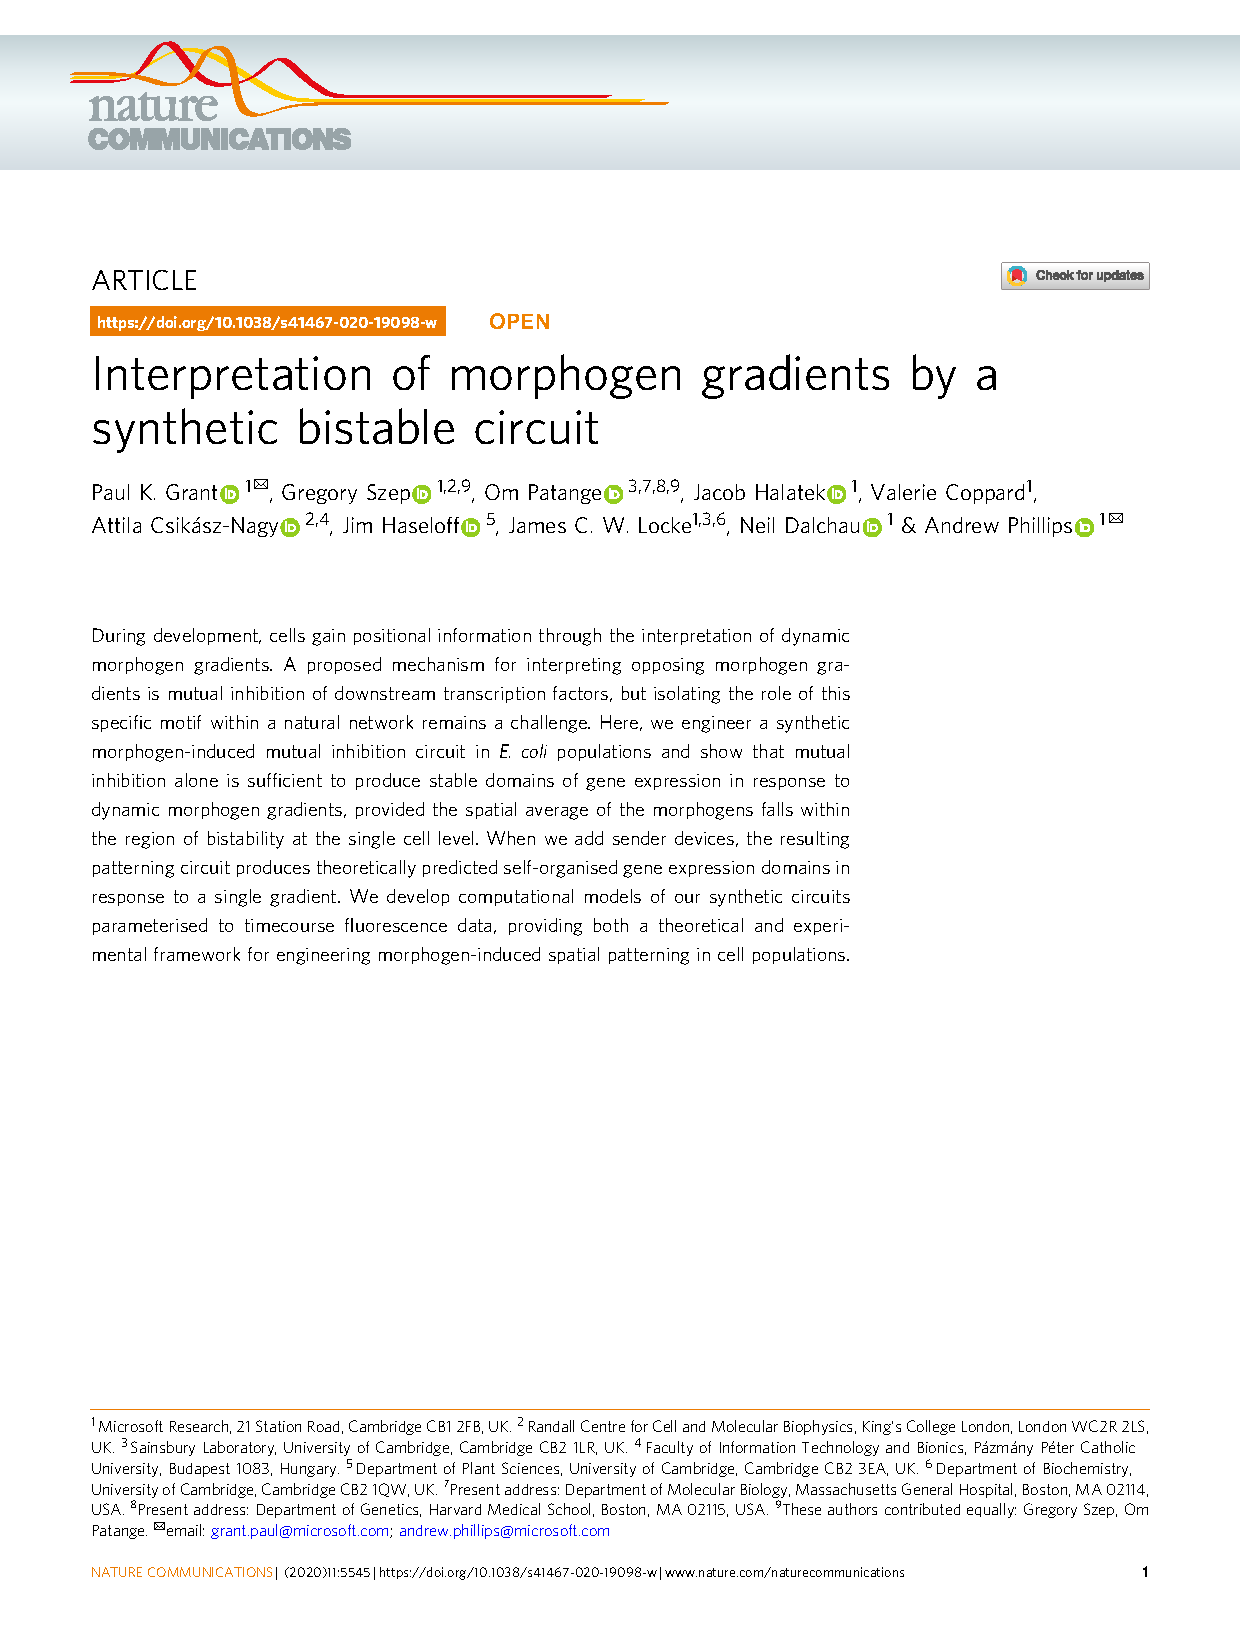
\includepdf[pages=-, offset=75 -75, addtotoc={
        2,section,1,Introduction,section:introduction,
        2,section,1,Results,section:results,
        2,subsection,2,Engineering mutual exclusivity,exclusivity,
        3,subsection,2,Mutual inhibition results in bistability,bistability,
        4,subsection,2,Hysteresis produces stable boundaries,boundaries,
        4,subsection,2,A secondary gradient creates self-organised domains,self-organisation,
        5,section,1,Discussion,section:discussion,
        6,section,1,Methods,section:methods,
        6,subsection,2,Plasmid construction,plasmids,
        6,subsection,2,Plate fluorometer assay,plates,
        6,subsection,2,Flow-cytometric analysis of hysteresis,flow,
        7,subsection,2,Microfluidics,microfluidics,
        7,subsection,2,Microfluidics microscopy,microscopy,
        7,subsection,2,Solid culture assays,cultures},
    addtolist={
        2, figure, {\textbf{A synthetic gene circuit for morphogen interpretation}. \textbf{a} Schematic representation of a developing embryo. Mutual inhibition of transcriptionfactors (cyan and yellow) downstream of antiparallel morphogen gradients (dark blue and orange) has been hypothesized to produce mutually exclusive domains of gene expression. \textbf{b} Morphogen gradients can be dynamic and transient, yet sharp, stable boundaries are observed between domains of gene expression. \textbf{c} A diagram of the Exclusive Receiver circuit. When 3O-C12-HSL (C12) levels are high, C12 binds to LasR, activating the expression of YFP and TetR, which represses the expression of LuxR, preventing expression of CFP and LacI. When 3O-C6-HSL (C6) levels are high, C6 binds to LuxR activating expression of CFP and LacI, which represses the expression of LasR, preventing expression of YFP and TetR. \textbf{d} Fluorescence output, measured in microplate fluorometer assays, of the Exclusive Receiver (top) and the Receiver (bottom) circuits represented as a ratio of CFP- (left) or YFP- (right) fluorescence to RFP fluorescence during exponential phase, cultured in the presence of the concentrations of C6 and C12 indicated. Data are representative of $n=3$ biological replicate experiments conducted on different days}, figure:overview,
        3, figure, {\textbf{Mutual inhibition produces bistability}. Cells transformed with the Exclusive Receiver circuit were conditioned in either 500 nM C6 \textbf{a}, or 500 nM C12 \textbf{b}, and then exposed to the combinations of concentrations of C6 and C12 indicated.  Cells were measured using flow cytometry and their normalized CFP minus YFP expressions were plotted. The region of bistability predicted by the parameterized model is the area within the red lines.  \textbf{c}, Microfluidics cultures of cells transformed with Exclusive Receiver circuit in changing combinations of signals.  Cells were grown for 3 hours in the presence of either 37 nM C6 (rows 1 and 2) or 100 nM C12 (rows 3 and 4). Then media was changed to 100 nM C12 + 37 nM C6 (rows 1 and 3) or 100 nM C12 (row 2) or 37 nM C6 (row 4) . Cells were imaged with a frame rate of (1 frame/10 minutes). Left panels are kymographs of the log-ratio of CFP expression per-cell to YFP expression per-cell, and fraction of cells as a heat map.  Histograms represent the populations at 3 hours (red) and 8 hours (blue).  Lines and shaded region represent the mean and standard deviation, respectively, over {n = 4  biological replicates performed on 4 different days.} Right panels are sample montages of cells switching state (rows 2 and 4) or exhibiting bistablity (rows 1 and 3); phase contrast and fluorescence channel ranges chosen for display. Scalebar=6$\mu$m.}, figure:bistability,
        5, figure, {\textbf{Formation of stable boundaries.} \textbf{a}, Endpoint fluorescence microscopy of Exclusive Receiver cells grown in transient gradients of signals (C12 diffusing from the left, C6 diffusing from the right) at the spatial average concentrations indicated and in the context of 10 $\mu$M IPTG throughout.  Representative examples (n=3 biological replicates performed on 3 different days) of a static boundary (left) and a moving boundary (right) \textbf{b}, Corresponding kymographs of CFP and YFP fluorescence (intensity) over time (y-axes, hours) at different spatial positions (x-axes, mm). If the location of the boundary (location of equal normalized CFP and YFP fluorescences, black lines) at the end of the timelapse minus its location when it became detectable ($\Delta\beta$, arrows) was less than 10\% of the domain size we considered the boundary stable.   \textbf{c}, Boundaries were evaluated as above at the signal concentrations indicated by letters. ‘S’ indicates equilibrium concentrations at which static boundaries were observed. ‘M’ indicates a moving boundary. 'N' indicates no boundary.  The color of the letter indicates which FP was dominant and red indicates neither FP dominant. \textbf{d}, Schematic representation of the concentrations of C6 and C12 experienced by cells at different points in physical space (cyan and yellow curves) as gradients diffuse to homogeneity.  Paler curves represent different timepoints.  If the spatial average concentrations lie within the region of bistability, the boundary will be static (S), otherwise the boundary will move (M) and will eventually be abolished as cells adopt either CFP or YFP expression.   $t_1$ and $t_2$ indicate timepoints considered in (e).  \textbf{e}, Corresponding schematic representing LasR expression, colored according to resultant fluorescent protein expression.  Dashed line indicates the location of an unstable local equilibrium. Red lines indicate the spatial location in which cells are exhibiting bistability.  In the case of a stationary boundary (S), the region of space containing cells exhibiting bistability expands to encompass all cells and their gene expression state is determined by their history.  In the case of a moving boundary (M), the region exhibiting bistability moves rightward and disappears and the domain becomes dominated by a single monostable state.}, figure:boundaries,
        6, figure, {\textbf{Addition of a Relay circuit creates self-organised domains of gene expression.} \textbf{a}, Circuit diagram of Exclusive Receiver cells co-transformed with a  Relay circuit  (P76-LasI) that responds to C6 by producing C12. \textbf{b}, Isogenic cells transformed with the circuit shown in (a) and grown for 24 hours in the presence of a gradient of C6 diffusing from the centre. Cells that experience high levels of C6 (central cells) will express CFP, LacI, and LasI, causing them to produce C12 but be unable to sense it.  Neighbouring cells (outer cells) that do not experience C6 will sense C12 and express YFP and TetR, resulting in mutually exclusive domains of gene expression.{ Cells also constitutively express mRFP1 via a genomic transgene. Image is representative of 3 biological replicates performed on 3 different days.} \textbf{c}, Quantitation of fluorescence along the dotted line in b. Cyan, yellow, and red indicate CFP, YFP, and RFP expression, respectively. \textbf{d}, Final timepoint of simulation shows a secondary gradient of C12 (orange) produced in response to the primary C6 gradient (dark blue).  Cyan and yellow indicate simulated CFP and YFP expression, respectively.  \textbf{e}, Final time point of simulation in C6-C12 space labelling points in physical space by their CFP and YFP expression (cyan and yellow points), and showing the production of C12 as vectors (red arrows) that move the spatial average (x) toward increasing C12}, figure:relay
}]{publications/double-exclusive.pdf}